% ════════════════════════════════════════════════════════════════════════════════
\section{Evaluation}
\label{sec:evaluation}

We demonstrate the system end-to-end across three scenarios: an L2 login
(first-ever login, password and TOTP); an L1 login (returning user from a
known IP, password only); and an L3 login (elevated risk, all three factors).
We additionally verify end-to-end tunnel connectivity and RBA score
correctness for each tier.
All scenarios start from a clean run of \texttt{scripts/setup.py} on a
fresh checkout.

% ─────────────────────────────────────────────────────────────────────────────
\subsection{Stack Setup}

\textbf{Prerequisites.}
The host must have \texttt{docker}, \texttt{docker compose} (v2), and
\texttt{wireguard-tools} installed, and the current user must be in the
\texttt{docker} group:
\begin{lstlisting}[language=bash,frame=none,basicstyle=\ttfamily\scriptsize]
sudo apt install docker.io docker-compose-v2 wireguard-tools
sudo usermod -aG docker $USER && newgrp docker
sudo modprobe wireguard   # verify kernel module is available
\end{lstlisting}
No Python dependencies are required on the host — every Python process runs
inside a container.

\textbf{Setup.}
\texttt{scripts/setup.py} is idempotent: it generates all secrets and the
server WireGuard keypair, builds the Docker images, starts the three
server-side containers (\texttt{vpn-idp}, \texttt{vpn-helpdesk},
\texttt{vpn-srvauthn}), and enrolls the test user \texttt{alice} with
password and TOTP.
The optional client container (\texttt{vpn-client}) is brought up
separately when running the authentication scenarios.
Figs.~\ref{fig:setup-top} and~\ref{fig:setup-bottom} show a clean run
and Fig.~\ref{fig:docker} confirms the containers are up with the
expected port bindings.

\begin{figure}[H]
  \centering
  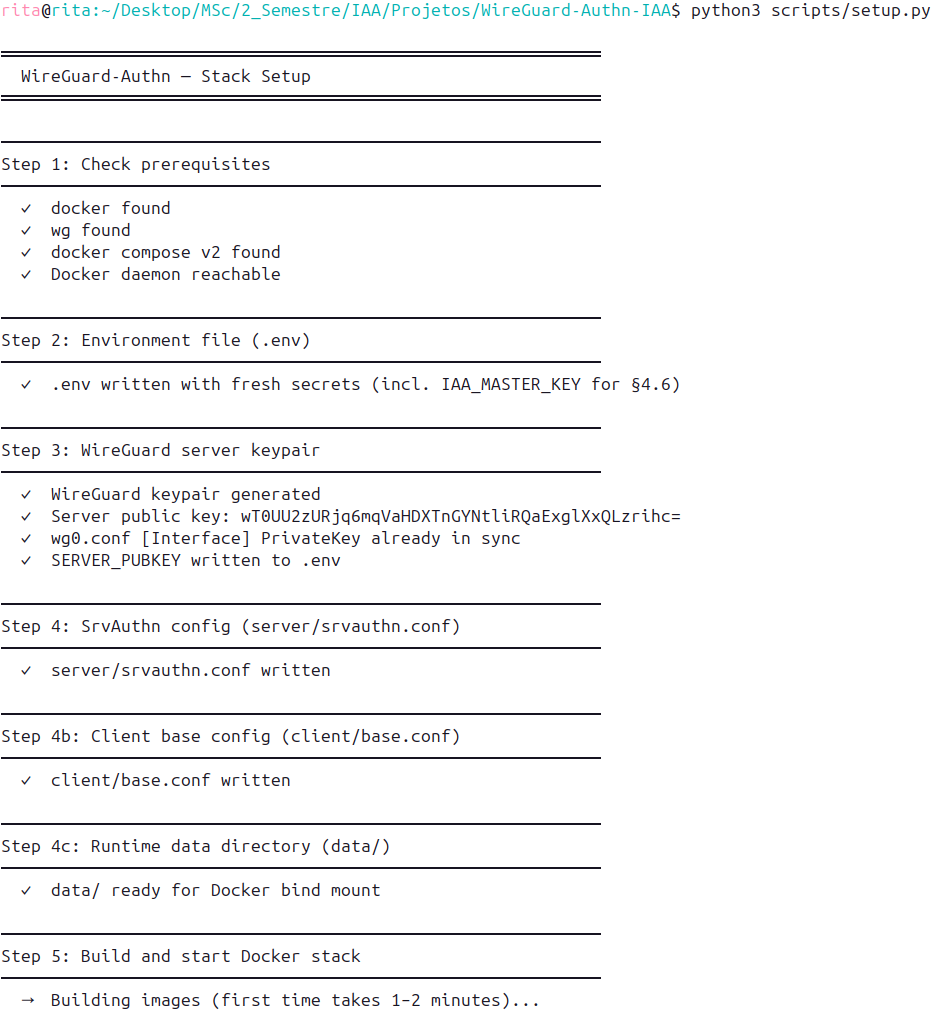
\includegraphics[width=1.0\columnwidth]{images/setup-top}
  \caption{\texttt{setup.py}: config and key generation (steps 1--4).}
  \label{fig:setup-top}
\end{figure}

\begin{figure}[H]
  \centering
  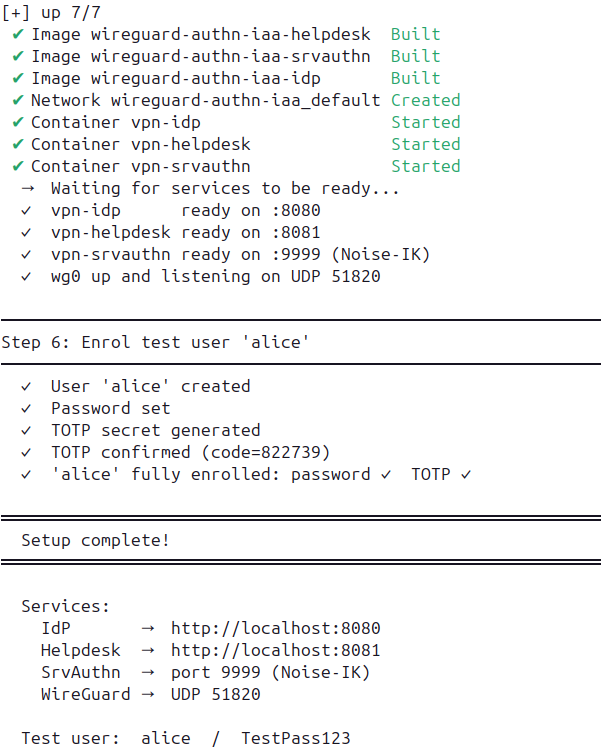
\includegraphics[width=1.0\columnwidth]{images/setup-bottom}
  \caption{\texttt{setup.py}: stack up and user enrolled (steps 5--6).}
  \label{fig:setup-bottom}
\end{figure}

\begin{figure}[H]
  \centering
  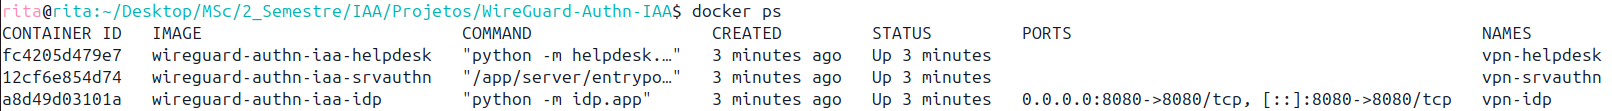
\includegraphics[width=1.0\columnwidth]{images/docker}
  \caption{Running containers after setup, with port bindings.}
  \label{fig:docker}
\end{figure}

% ─────────────────────────────────────────────────────────────────────────────
\subsection{Helpdesk Enrolment}

The helpdesk at \texttt{http://localhost:8081} manages all three factors
per user (Figs.~\ref{fig:helpdesk-users} and~\ref{fig:helpdesk-profile}).
The TOTP QR code and FIDO2 registration prompts are shown in
Figs.~\ref{fig:totp-enrol} and~\ref{fig:fido2-reg}
(Section~\ref{sec:mfa}).
For the FIDO2 enrolment, the virtual FIDO device
(\texttt{sudo python3 virtual\_fido/src-fido/virtual\_fido.py}) must be
running.

\begin{figure}[H]
  \centering
  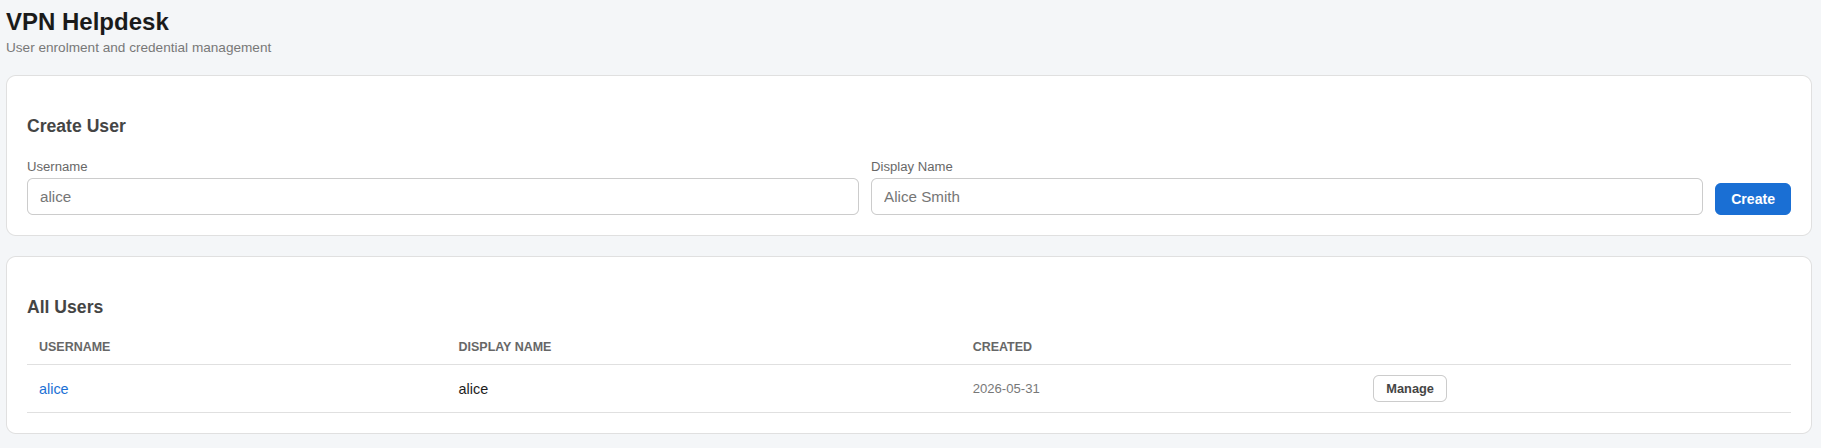
\includegraphics[width=1.0\columnwidth]{images/helpdesk-users}
  \caption{Helpdesk user list.}
  \label{fig:helpdesk-users}
\end{figure}

\begin{figure}[H]
  \centering
  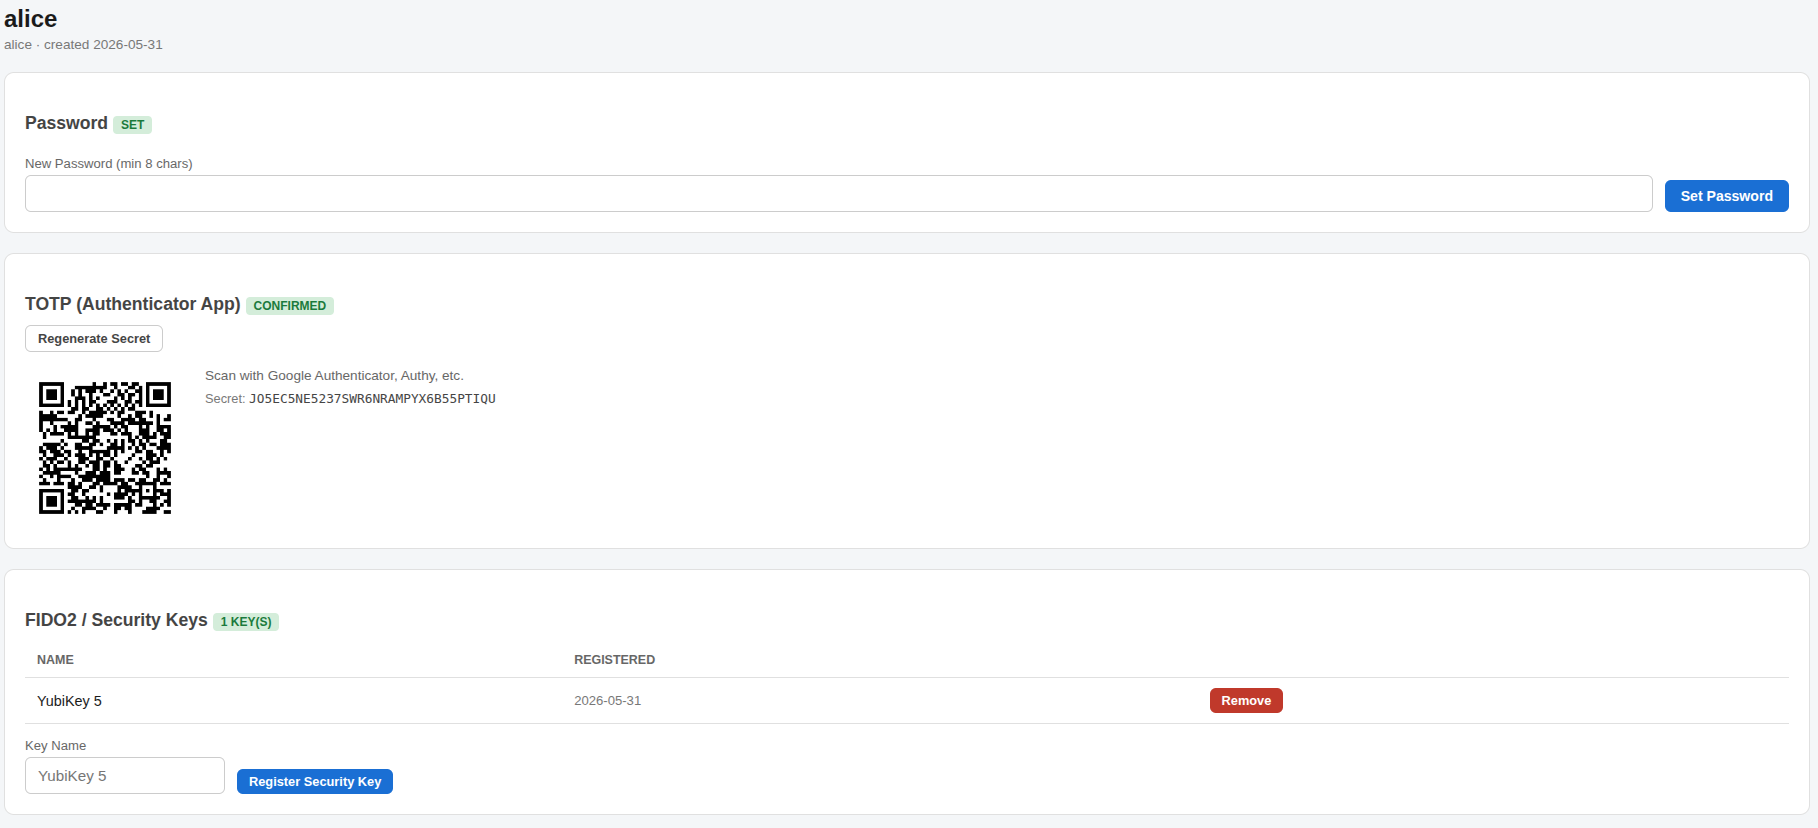
\includegraphics[width=1.0\columnwidth]{images/helpdesk-profile}
  \caption{Per-user panel, all factors enrolled.}
  \label{fig:helpdesk-profile}
\end{figure}

% ─────────────────────────────────────────────────────────────────────────────
\subsection{L2 Authentication: Password and TOTP}

To reproduce, bring up the optional client container and run
\texttt{userauthn.py} inside it:
\begin{lstlisting}[language=bash,frame=none,basicstyle=\ttfamily\scriptsize]
docker compose --profile client up -d --build client
docker exec vpn-client python3 -u /workspace/client/userauthn.py \
  --interface wg0 --username alice \
  --config /workspace/client/base.conf --proxy-host 0.0.0.0
\end{lstlisting}

A first login from a clean state scores 0.30 (the first-ever-login
signal), placing \texttt{alice} at tier L2: password and TOTP.
\texttt{UserAuthn} generates the PSK, opens the Noise-IK tunnel, and
prints the device code (Fig.~\ref{fig:userauthn-start}).

\begin{figure}[H]
  \centering
  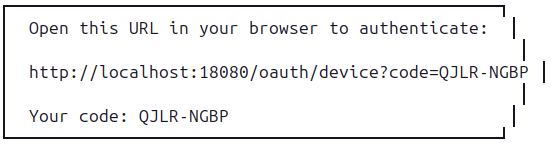
\includegraphics[width=1.0\columnwidth]{images/userauthn-start}
  \caption{\texttt{UserAuthn} terminal at authentication start.}
  \label{fig:userauthn-start}
\end{figure}

The browser opens the OAuth device page with the code pre-filled
(Fig.~\ref{fig:browser-device}).

\begin{figure}[H]
  \centering
  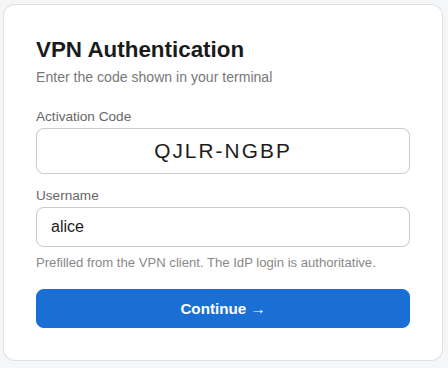
\includegraphics[width=0.8\columnwidth]{images/browser-device}
  \caption{OAuth device page --- code pre-filled via redirect URI.}
  \label{fig:browser-device}
\end{figure}

The user completes the password factor (Fig.~\ref{fig:mfa-password})
and the TOTP factor (Fig.~\ref{fig:mfa-totp}).
On success the browser shows the completion page
(Fig.~\ref{fig:auth-complete-l2}).

\begin{figure}[H]
  \centering
  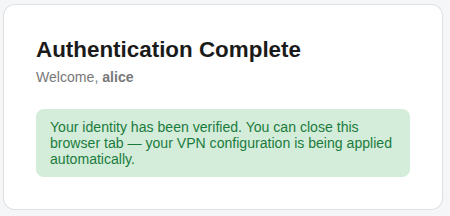
\includegraphics[width=0.9\columnwidth]{images/auth-complete-l2}
  \caption{Authentication complete after password and TOTP.}
  \label{fig:auth-complete-l2}
\end{figure}

The terminal then shows the leased tunnel IP, confirming the WireGuard
interface is up (Fig.~\ref{fig:vpn-connected-l2}).

\begin{figure}[H]
  \centering
  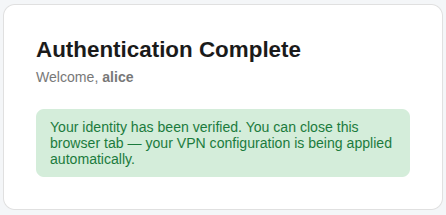
\includegraphics[width=0.9\columnwidth]{images/vpn-connected-l2}
  \caption{Client terminal after a successful L2 login.}
  \label{fig:vpn-connected-l2}
\end{figure}

% ─────────────────────────────────────────────────────────────────────────────
\subsection{L1 Authentication: Password Only}

After the L2 login above, \texttt{alice}'s IP is recorded in
\texttt{rba\_ip\_history}.
A second login from the same machine during normal hours with no recent
failures scores 0.00 — no signal fires — placing \texttt{alice} at tier
L1: password only.
To reproduce: immediately after the L2 session, run
\texttt{python3 scripts/teardown.py --session} to clear the WireGuard peer
and session tables while preserving \texttt{rba\_ip\_history}, then run
\texttt{userauthn.py} again.
The browser shows only the password factor (Fig.~\ref{fig:mfa-l1-password});
the TOTP step does not appear.

\begin{figure}[H]
  \centering
  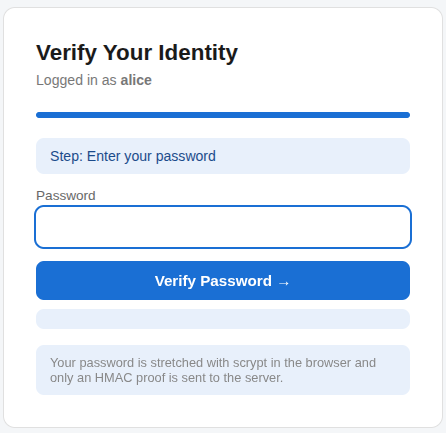
\includegraphics[width=0.8\columnwidth]{images/mfa-l1-password}
  \caption{Password-only factor page during an L1 login.}
  \label{fig:mfa-l1-password}
\end{figure}

The tunnel comes up on completion (Fig.~\ref{fig:auth-complete-l1}).

\begin{figure}[H]
  \centering
  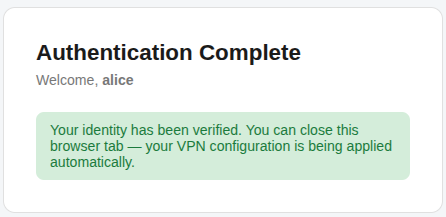
\includegraphics[width=0.9\columnwidth]{images/auth-complete-l1}
  \caption{Authentication complete after password only (L1).}
  \label{fig:auth-complete-l1}
\end{figure}

% ─────────────────────────────────────────────────────────────────────────────
\subsection{L3 Authentication: Password, TOTP, and FIDO2}
\label{sec:eval-l3}

The FIDO2 factor is required at tier L3, reached when the risk score is
at least 0.60.
To reproduce: reset the DB auth tables (\texttt{teardown.py --reset}),
ensure \texttt{alice} has a FIDO2 credential enrolled, then make
\emph{four failed password attempts in separate sessions} before the real
login (the risk score is computed at session start, so only failures from
prior sessions count toward it).
Four failures add $4 \times 0.10 = 0.40$ to the first-login baseline of
$0.30$, giving a score of $0.70 \geq 0.60$.
The virtual FIDO device must be running.
After password and TOTP pass, the browser presents the FIDO2 assertion
dialog (Fig.~\ref{fig:mfa-fido2-login}).

\begin{figure}[H]
  \centering
  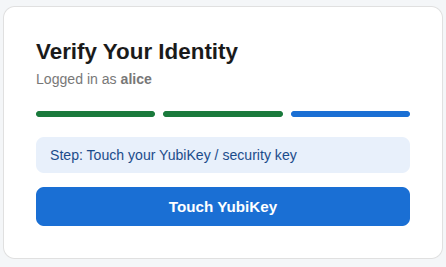
\includegraphics[width=0.85\columnwidth]{images/mfa-fido2-login}
  \caption{FIDO2 factor step during an L3 VPN login.}
  \label{fig:mfa-fido2-login}
\end{figure}

On success the completion page appears (Fig.~\ref{fig:auth-complete-l3}).

\begin{figure}[H]
  \centering
  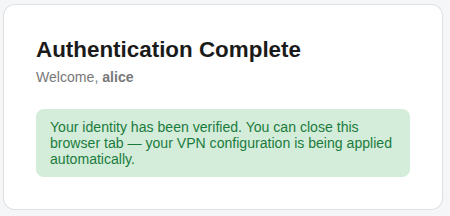
\includegraphics[width=0.9\columnwidth]{images/auth-complete-l3}
  \caption{Authentication complete after all three L3 factors.}
  \label{fig:auth-complete-l3}
\end{figure}

The terminal confirms the tunnel is up (Fig.~\ref{fig:vpn-connected-l3}).

\begin{figure}[H]
  \centering
  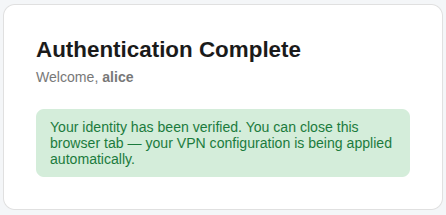
\includegraphics[width=0.9\columnwidth]{images/vpn-connected-l3}
  \caption{Client terminal after a successful L3 login.}
  \label{fig:vpn-connected-l3}
\end{figure}

% ─────────────────────────────────────────────────────────────────────────────
\subsection{Server-Side Verification}

After any successful login, \texttt{wg show wg0} inside the
\texttt{vpn-srvauthn} container lists the provisioned peer with its
tunnel IP, pre-shared key, and most recent handshake timestamp
(Fig.~\ref{fig:wg-server}).

\begin{figure}[H]
  \centering
  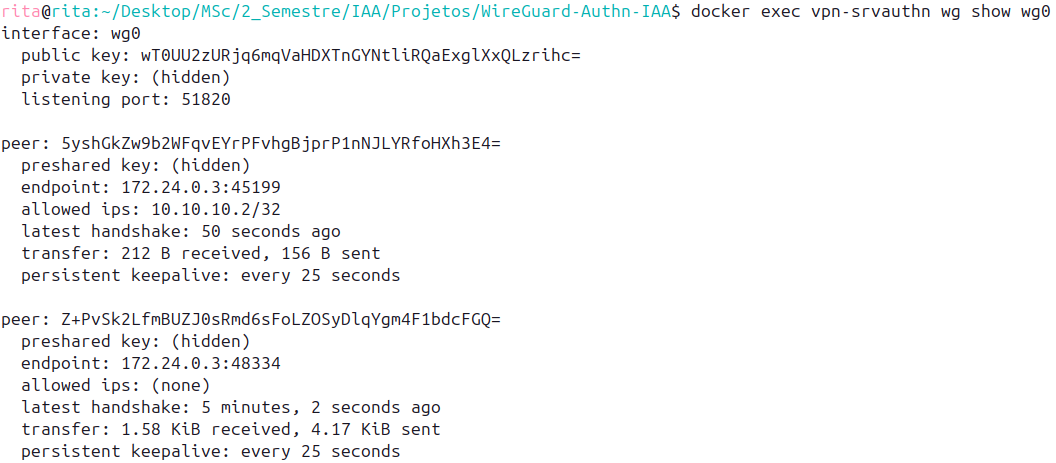
\includegraphics[width=1.0\columnwidth]{images/wg-server}
  \caption{Server-side \texttt{wg show wg0} after provisioning.}
  \label{fig:wg-server}
\end{figure}

A \texttt{ping} from the client container to the server tunnel address
\texttt{10.10.10.1} confirms that the tunnel carries traffic end-to-end
(Fig.~\ref{fig:ping}).

\begin{figure}[H]
  \centering
  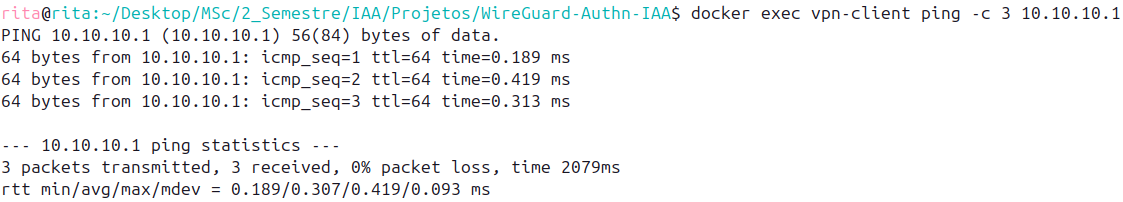
\includegraphics[width=1.0\columnwidth]{images/ping}
  \caption{End-to-end ping through the WireGuard tunnel.}
  \label{fig:ping}
\end{figure}

% ─────────────────────────────────────────────────────────────────────────────
\subsection{RBA Score Verification}

The RBA engine logs the computed score and active signals on every login.
A first-ever login fires only the \texttt{first\_login} signal
(score~0.30, tier~L2).
A returning user from a known IP during normal hours fires no signals
(score~0.00, tier~L1).
A first login preceded by four failed attempts in previous sessions
accumulates $0.30 + 4 \times 0.10 = 0.70$, exceeding the L3 threshold
of 0.60.
Fig.~\ref{fig:rba-scores} shows the IdP log output for all three
scenarios together.

\begin{figure}[H]
  \centering
  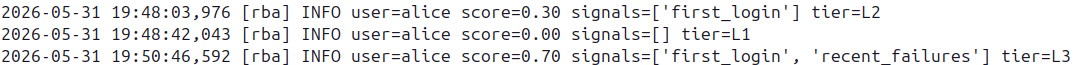
\includegraphics[width=1.0\columnwidth]{images/rba-scores}
  \caption{IdP log output confirming the RBA score and tier for each scenario.}
  \label{fig:rba-scores}
\end{figure}

% ─────────────────────────────────────────────────────────────────────────────
\subsection{Discussion}

The Noise-IK handshake and WireGuard bring-up complete in well under a
second on loopback; \texttt{wg-quick up} takes roughly 200~ms.
The dominant wall-clock cost is the user completing MFA in the browser.
The OAuth polling interval is 5~s, so the maximum additional delay between
``MFA done'' and ``tunnel active'' is one poll cycle plus the bring-up
time, well within acceptable limits for a VPN login.

The risk score is deterministic given a fixed DB state, so every scenario
is fully reproducible.
The RBA log output provides direct evidence that the score and tier
assignment match the signal weights described in Section~\ref{sec:rba},
with no manual inspection of internal state required.
